\documentclass{article}
\usepackage[english]{babel}
\usepackage[utf8]{inputenc}
\usepackage{xspace}
\usepackage{graphicx,graphics} 
\usepackage{color}
\usepackage{amsmath}
\usepackage{amsfonts}
\usepackage{amssymb}
\usepackage{amsthm}

\usepackage{longtable}
\usepackage{complexity}

\newcommand\rmatching{$\cal R$-matching\xspace}
\newcommand\mdelay{$\cal M$-delay\xspace}
\newcommand\matchedgraph{{\bf matched graph}}
\begin{document}


\graphicspath{{figures/}}
\newtheorem{rem}{Remarque}
\newtheorem{proposition}{Proposition}
\newtheorem{theorem}{Theorem}
\newtheorem{fact}{Fact}
\newtheorem{lemma}[theorem]{Lemma}
\newtheorem{definition}{Definition}

\title{Latency for periodic multicasting}

\newcommand{\todo}[1]{}
\renewcommand{\todo}[1]{{\color{red} TODO: {#1}}}
 
\author{DB, CC, OM, YS, MG}

  % ?

\maketitle

 
\section{Introduction}

\subsection{Context}
Mobile networks are controled by many radio stations, composed of 2 major parts : 
\begin{enumerate}
 \item Base Band Units (BBU) : are resonsible for computing the signals, and communicate with the core network.
 \item Remote Radio Head (RRH) : are the antennas and have only to communicate with the mobile devices.
\end{enumerate}
The part of the network between BBU and the core network is called backhaul.

The operators are searching for a way to dissociate BBU from RRH, and regroup many BBU in some data centers, that would allow easyer updates and 
maintenance.
Nevertheless such a splitting enforce hard throughput and latency constraints on the communication network between BBU and RRH. This part of the network is called fronthaul.

In this article, we will work on latency constraints in fronthaul.

\subsection{Definitions}
We consider a directed graph $G=(V,A)$ with two non intersecting subsets of vertices: a subset $L$ of nodes which are called \emph{leaves} and a subset $S$ of nodes which are called \emph{sources}.  
We denote by ${\cal L}$ the cardinal of $L$. The digraph $G$ models the network, $S$ the possible BUU and $L$ the set of RRH.
Each arc  $(u,v)$ in $A$ is caracterised by an integer delay $Dl(u,v) \geq 1$ representing the time taken by the signal to go from $u$ to $v$
by using this arc.  

We'll consider $G=(V,A)$ and $G^r=(V,A^r)$ wherein the set of vertices is the same and $A^r$ represents the edges of $A$ directed in the other way. 
The delay $Dl(u,v)$ represents the weight of the arcs between $u$ and $v$.\newline

\begin{tabular}{cc}
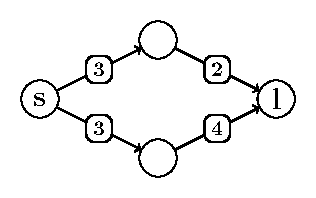
\includegraphics[scale=0.8]{Fig2.pdf} & 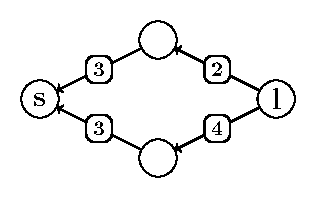
\includegraphics[scale=0.8]{Fig3.pdf}\\
 $G=(V,A)$ & $G^r=(V,A^r)$\\
\end{tabular}\newline
Note that there is a special case in which the graph may have oriented cycles (optical ring topologie),
otherwise, there is no oriented cycles and all the properties are availables.

A route $r$ is a sequence of arcs $a_0, \ldots , a_{n-1}$, with $a_i=(u_i,u_{i+1}) \in A$ such that $u_0 \in S$ and $u_n \in L$.
The {\em latency} of a vertex $u_i$ in $r$, with $i \geq 1$, is defined by $$\lambda(u_i,r)= \sum\limits_{0 \leq k <i} Dl(a_k)$$ We also define $\lambda(u_0,r)=0$.
The latency of the route $r$ is defined by $\lambda (r)= \lambda (u_n,r)$. In graph theory, a route is a simple path in the graph, and its latency is its weight. 
Consider that the term ``route $r$`` denote the route itself but also its source node $u_0$ in $S$ an its leave node $u_n$ in $L$.

A {\bf routing function} ${\cal R}$ is an application associating a route ${\cal R}(s,l)$ to each couple $(s,l) \in S \times L$ in $G$. 
A {\bf ${\cal R}$-matching} of $S$ in $L=\{l_0, \ldots , l_{{\cal L}-1}\}$ is a set of ${\cal L}$ routes $\rho =\{r_0, \ldots ,r_{{\cal L}-1}\}$.
It is a bijection of $S$ in $L$.
We assume that we have as many source nodes node as we have leaves. This means that each source or leave node belongs to exactly one route in $\rho$.
Moreover $\rho$ satisfies the \emph{coherent routing} property: the intersection of two routes must be a path.

%The ${\cal R}$-matching $\rho$ defines a subgraph of $G$ wich is the union of all paths in $\rho$ that we call the \emph{routing graph} and that we denote by $G_{\rho}$. 



For each arc $(u,v) \in A$, we denote by ${\rho}(u,v)$ the subset of routes of $\rho$  containing $(u,v)$.
We define the load of an arc $(u,v)$ as the number of routes that use this arc thus : $load(u,v) = |\rho(u,v)|$.

The quintuplet $N=\{G,S,L,R,\rho\}$ defines a \matchedgraph. We call $N^r$ the quintuplet $\{G^r,S,L,R,\rho^r\}$, 
where $\rho^r$ is the \rmatching obtained using the same routes, with inverted arcs.

Let $P>0$ be an integer called {\em period}. 
A $P$-periodic affectation of N, a matched graph consists in a set  ${\cal M}=\{m_0, \ldots ,m_{{\cal L}-1}\}$ of ${\cal L}$ integers that we call \emph{offset}. 
Each time window is divided in $P$ slots and the number $m_i$ represents the slot number used by the route $r_i$ at its source.
We define the time slot used by a route $r_i$ at any vertex $v$ of the route by $$t(v,r_i) = m_i+\lambda(u,r_i)) \mod P.$$
A $P$-periodic affectation must have no {\em collision} between two routes in $\rho$, that is $\forall r_i, r_j \in \rho, i \ne j$, two routes intersecting in u,
and containing the same arc $(u,v)$, we have $$t(u,r_i)\ne t(u,r_j) .$$

We define by $\alpha(u,r_i,r_j) = | \lambda(u,r_i)-\lambda(u,r_j)|$. This item will be useful later, when we'll introduce Route Conflict Graphs.
 

%Giving a $P$-periodic affectation $\cal M$ of $\rho$, for any route $r^i \in \rho$, we call $\cal M$-delay of  $r^i$ the integer $d_{\cal M}(r^i)=\lambda(r^i)+m_i$. We also call {\bf $\cal M$-delay} of ${\cal R}$ the maximum $\cal M$-delay of a route in $\rho$.\\

Notice that the notion of $P$-periodic affectation \textbf{is not monotone} with regard to $P$. 
Indeed, we can build a {\bf ${\cal R}$-matching} of a graph, with $l$ routes $r_1, \dots, r_l$ which all intersect two by two and
such that if $r_i$ and $r_j$ have $v$ as first common vertex we have $\lambda(v,r_i) - \lambda(v,r_j)=1$.
Therefore there is a $2$-periodic affectation by setting all $m_i$ to $0$.

\begin{tabular}{cc}
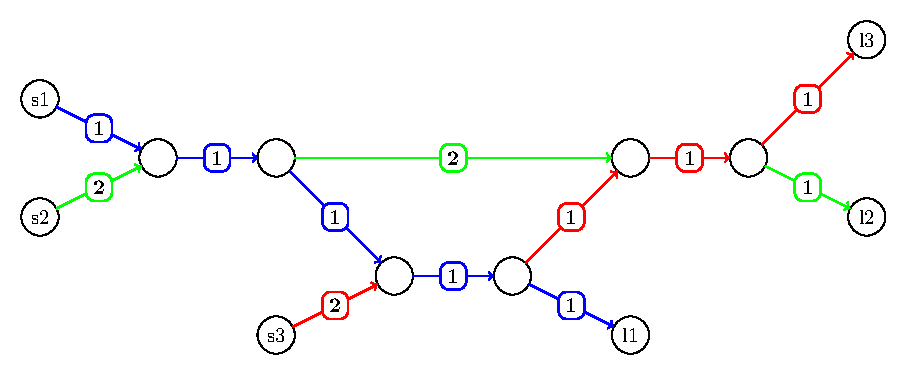
\includegraphics[scale=0.5]{Fig5.pdf} & 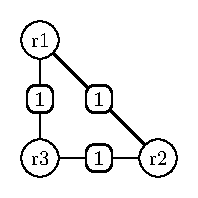
\includegraphics[scale=1]{Fig7.pdf}\\
 $\lambda(v,r_i) - \lambda(v,r_j)=1$ & Conflict graph\\
\end{tabular}\newline

On the other hand if we set all $\lambda(v,r_i) - \lambda(v,r_j)=P$, there is no $P$-peridodic affectation if $P<l$.

\begin{tabular}{cc}
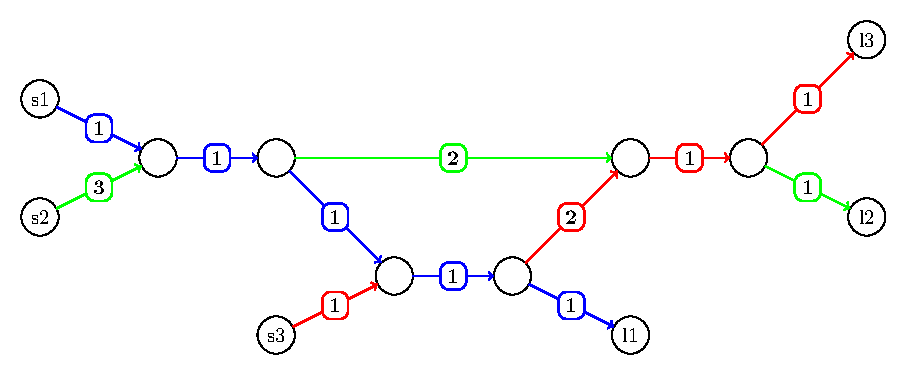
\includegraphics[scale=0.5]{Fig6.pdf} & 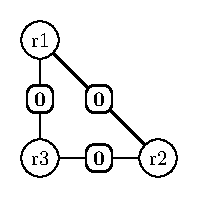
\includegraphics[scale=1]{Fig8.pdf}\\
 $\lambda(v,r_i) - \lambda(v,r_j)=2$ & Conflict graph\\
\end{tabular}\newline
\begin{center}
 Here for P=2, there is no P-Periodic affectation.
\end{center}

Therefore if we choose $P$ odd and $l=P+1$, there is no $P$-peridodic affectation but modulo $2$ all $\lambda(v,r_i) - \lambda(v,r_j)$
are equal to one thus we have a $2$-periodic affectation. 
 


\subsection{Real Network Topologies}

To illustrate we consider an basic network topologie, composed of some base stations, represented by source nodes $S$, all connected to the same switch,
which will be a vertex, connected himself to another vertex, corresponding to a switch, connected to some leave nodes $L$ representing the Antennas.

\begin{center}
 
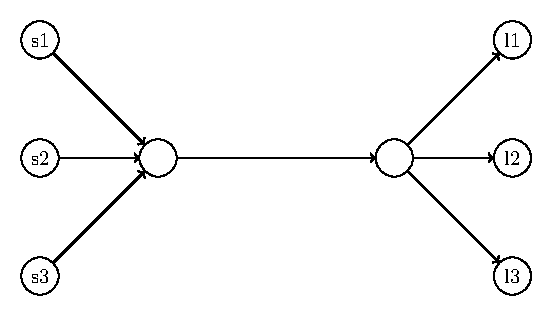
\includegraphics[scale=1]{Fig4.pdf}\\
Example of topologie 1.
\end{center}

\todo{ajouter les autres topologies}

\subsection{Fronthaul networks}

The application we address here by studying the problems defined above is the following. Consider fronthaul network in which source nodes in $S$ represent computing units in data centers,
each one able to do a remote process for base stations modeled by leaves node in $L$. Consider a ${\cal R}$-matching $\rho$ of $S$ in $L$. Consider a leave $l$, its dedicated source node $s$
and $R(l,s)$ the route from $l$ to $s$ in $R$. We consider a $P$-periodic affectation of $\rho$, and also another $P$-periodic affectation of $\rho^{r}$, the $R$-matching
obtained by considering $G^r$, using the same routes in opposite direction. The periodic process is then the following one:
\begin{enumerate}
 \item During each period of duration $P$, leave $l$ sends a message to $s$, using $R(l,s)$ from $l$ to $s$. Note that this sending is periodic but can use any time slot in the time window.
 \item When $s$ receives this message, it makes a computation to answer $l$.
 \item Then source $s$ sends a message to $l$ using $R(s,l)$.
\end{enumerate}
On source nodes, between the end of computation time and the emission time of the message (given by the $P$-periodic affectation), there is a waiting time. 
We define by $\omega : r \rightarrow \mathbb{N}$ the waiting time of a route $r$ in the ${\cal R}$-matching considered, i.e. the time during while the
message is ''sleeping``, waiting to be sent through the network.


Source and leave nodes periods have to be the same. Indeed, leave nodes have to receive a message at every period, so source nodes have to send a message at every same period.
So, we will find two P periodic affactations from the same P in both ways. 
If the message have to be buffered, we want to do it in souces nodes.
We define by $\theta$ the computation time required at the source node before sending an answer to it's leave node.

Let's Call $T (r)$ the process time on a route $r$: $$ T (r) = 2\lambda (r) + \omega (r) + \theta(r)$$


 
 We consider 3 main problems:\\

\noindent {\bf Problem  Periodic Routes Assignment (PRA)} 

\noindent {\bf Input:} matched graph $N$, integer $P$.

\noindent {\bf Question:} does there exist a $P$-periodic affectation of $N$ ?

\noindent {\bf Optimisation goal:} minimizing $P$.\\

This problem is our basic problem. We need to find the offset for each routes such that there is no collision between the signals emitted by sources at any nodes in the graph.\\

\noindent {\bf Problem  Network Periodic Assignment (NPA)} 

\noindent {\bf Input:} $G=(V,A)$, $S$, $L$,  a routing $\cal R$, integers $P$

\noindent {\bf Question:} does there exist  a ${\cal R}$-matching $\rho$ of $S$ in $L$ such that there exists a $P$-periodic affectation $\cal M$ of $\rho$ ?

\noindent {\bf Optimisation goal:} minimizing $P$.\\

This problem is the same problem than PRA in which is added the liberty to find the $R-matching$.

In our network application $\theta$ is set to 2,6ms, the period P is 1ms and T(r) must be less or equal than 3ms.

So P and the $R-matching$ are given, we do not need to minimize P and P is great enough to carry the dataload.
The real network problem is the following:\\

\noindent {\bf Problem Periodic Assignment for Low Latency(PALL)} 

\noindent {\bf Input:} matched graphs $N$,$N^r$, integer $P$, $ T_{max}$, $\theta$.

\noindent {\bf Question:} does there exist a $P$-periodic affectation $\cal M_1$ of $N$ and A $P$-periodic affectation $\cal M_2$ of $N^r$, considering $M_1$ and $\theta$,
such that $\forall r \in \rho T(r) \le T_{max}$.

\noindent {\bf Optimisation goal 1:} minimizing $\sum_{r \in \rho}  T(r)$.\\

By minimizing the sum of all the routes, we allow a better global Quality of Service threw the network.

\noindent {\bf Optimisation goal 2:} minimizing max(T(r)).\\

We have to find a $P$-periodic affectation of $G^r$ (solving PRA), then to find the $P$-periodic affectation of $G$ considering the computation time. 
The offsets of this second P-periodic affectation will correspond to waiting times.

\section{Reservation and PRA}


Here we study the impact of the parameter $\delta$ (the reservation) in the PRA problem. 
Ideally we would like to get rid of it and find optimal solutions for any $\delta>O$
from a solution with $\delta = 0$ for the same graph. 
The most natural idea is to transform each slot in a time window into $(\delta+1)$ slots to each and we multiply all offsets by $(\delta+1)$ 
to get a periodic affectation of period multiplied by $(\delta+1)$. Conversely, we could take any solution for $\delta>O$ and divide the offsets and the period by 
$\delta +1$. Both ideas do not work because when we change the period the delays modulo the new period may change and not all in the same way.

\todo{Exemple ou ça marche bien: la clique }

\todo{Donner des exemples de pourquoi ça ne marche pas}

On the other hand, while modelling the problem, we arbitrarily chose what is of size one, thus we can always 
chose it so that it takes into account the reservation (we should validate this remark with Olivier). The problem is the 
fractional values we get for the delays (already for $\delta =0$). By rounding them we could get transmission which seem at distance $1$ 
in the time window but which are arbitrarily close. This could be a justification to always have $\delta =1$.  



% 
% \begin{lemma}
%  Let $G=(V,A)$, $S$, $L$, a routing $\cal R$ and a ${\cal R}$-schedule $\rho$ of $S$ in $L$. If there is a $P$-periodic affectation 
%  for $PRA$ on this input with $\delta =0$ then for any $\delta >0$ we have a $(\delta+1)P$-periodic affectation.
% \end{lemma}
% \begin{proof}
%  Let  $\{m_0, \ldots ,m_{{\cal L}-1}\}$solution for $\delta =0$
% \end{proof}




\todo{On devrait mettre ça après le conflict system, car c'est plus simple à comprendre avec ce formalisme je pense.}


\section{Complexity results}


The \emph{conflict depth} of a $\cal R$-matching is the maximum number of arcs in a route which are 
shared with other routes. In other words it is the maximal number of potential conflicts along one route. 
The \emph{load} of a $\cal R$-matching is the maximal number of routes which share the same edge.
It is clear that a $P$-peridodic affectation must satisfy that $P$ is larger or equal to the load.

We give two alternate proofs that PRA is $\NP$-complete.
The first one works for conflict depth $2$ and is minimimal in this regards since we later prove that for conflict depth one,
it is easy to solve PRA. The second one reduces the problem to graph coloring and implies inapproximability. 
In all this section the reservation \textbf{$\delta$ is assumed to be $0$}.

\todo{ajouter des références à des problèmes de réseau similaires et de transport en commun qui sont également NP complets.}

We define two characteristic graphs associated to a $\cal R$-matching.

\begin{definition}[Edge Conflict Graph]
  The Edge Conflict Graph (ECG) of a \rmatching of a digraph $G=(V,A)$ is the graph $G'=(V',E')$ such that 
  a vertex of $V'$ is an arc of $A$ with a load greater than one. There is an edge between two vertices of $V'$
  if and only if there is a route which contains the two arcs of $A$ corresponding to the two vertices.
  
  This graph can be oriented so that an edge is oriented as the path in a route it represents and
  we can associate as weight to this edge, the delay of the corresponding path.
\end{definition}


\begin{definition}[Route Conflict Graph]
The Route Conflict Graph (RCG) of a \rmatching of a graph $G=(V,E)$ is the graph $G'=(V',E')$ where 
the vertices of $V'$ are the routes of the  \rmatching and there is an edges between two vertices
corresponding to two routes if and only if they share an edge.

We fix an arbitrary ordering on the elements of $V'=\{v_1,\dots,v_n\}$.
We can associate a weight to each edge $(v_i,v_j)$. Assume that $i < j$, 
and that the routes $r_i$ and $r_j$ corresponding to $v_i$ and $v_j$ have $u$ as first common vertex.
Then the weight of $(v_i,v_j)$ is $\lambda(u,r_i) - \lambda(u,r_j)$.
\end{definition}


\todo{Dire comment une solution à PRA s'exprime dans ces graphes avant de faire les preuves de NP-complétude}


\begin{proposition}
Problem PRA is $\NP$-complete, for a routing with conflict depth two.
\end{proposition}
 \begin{proof}
  Let $G=(V,E)$ be a graph and $d$ its maximal degree, we want to determine whether it is edge colorable
  with $d$ or $d+1$ colors. We reduce this edge coloring problem to PRA: we define a graph $H$, for each 
  $v \in V$ there are two vertices connected by an edge $(v_1,v_2)$ and none of these edges are incident.
  Those edges are of weight $1$.
  The schedule $\rho$ of $H$ is the set of routes $s_{u,v},u_1,u_2,v_1,v_2,l_{u,v}$ for each edge $(u,v)$ in $G$. The weight of  
  the two new edges is $d(d+1)-1$. The parameter $\delta$ is set to $0$.
  
  Let $\phi$ be an edge coloring with $k$ colors of $G$. We can build a $k$ periodic schedule 
  by assigning to the source $s_{u,v}$ of each route an offset  of $\phi(s_{u,v})$. Indeed, 
  if two routes $r_1$ and $r_2$ share the same edge, say $(v_1,v_2)$ then they represent two edges $e_1$ and $e_2$ of $G$ incident  
  to the vertex $v$. Therefore $\lambda(v_1,r_1) = \phi(e_1) \mod k$ because the delays of the edges before $v_1$ sum to $d(d+1)$ or 
  $2(d(d+1))$ which are equal to $0$ modulo $k$ since $k=d$ or $k=d+1$. Thus $\lambda(v_1,r_1) - \lambda(v_1,r_2) \mod k = \phi(e_1) - \phi(e_2) \mod k$
  and $\lambda(v_1,r_1) - \lambda(v_1,r_2) \mod k > 0$ since $\phi(e_1) \neq \phi(e_2) $.
  
  Now consider a $k$-periodic affectation of $\rho$. For each $(u,v)$ in $G$, we define $\phi(u,v)$ to be the offset of the route
  beginning at $s_{u,v}$. For the same reasons as in the last paragraph, $\phi$ is an edge coloring with $k$ colors.
  Therefore we have reduced edge coloring which is $\NP$-hard~\cite{holyer1981np} to PRA which concludes the proof. 
 \end{proof}


\begin{theorem}
 Problem PRA cannot be approximate within a factor $n^{1-o(1)}$ unless $\P = \NP$ even when the load is two
 and $n$ is the number of vertices.
\end{theorem}

\begin{proof}
 We reduce PRA to graph coloring. Let $G$ be a graph instance of the $k$-coloring problem. 
 We define $H$ in the following way: for each vertex $v$ in $G$, there is a route $r_v$ in $H$.
 Two routes $r_v$ and $r_u$ share an edge if and only if $(u,v)$ is an edge in $G$ and this edge is only in this two routes. 
 We put weight inbetween shared edges in a route so that there is a delay $k$ between two such edges. 
 
 As in the previous proof, a $k$-coloring of $G$ gives a $k$-periodic schedule of $H$
 and conversly. Therefore if we can approximate the value of PRA  within a factor $f$,
 we could approximate the minimal number of colors needed to color a graph within a fator $f$, 
 by doing the previous reduction for all possible $k$. The proof follows from the hardness of approximability
 of finding a minimal coloring~\cite{zuckerman2006linear}.
\end{proof}


In particular, this reduction shows that even with small maximal load, the 
minimal period can be large.


\todo{By using ideas similar to Vizing theorem, we may prove the following theorem for graph of congestion depth $2$.
In the proof there is just an analog of the lemma used to prove Vizing theorem, we should try to complete the proof.
Also can we say something similar when the congestion depth is larger ? }


\begin{proposition}
The solution to PRA is either the load or the load plus one.
Moreover, a solution of  load plus one can be built in polynomial time.
\end{proposition}

\begin{proof}
 First we define an alerning path and how it characterizes an optimal solution of PRA.
 Let $v$ be a vertex of degree $d$ in the congestion graph (to be defined). We assume that the 
 coloring of the edges is optimal (to define in the case of a congestion graph). 
 The color $\alpha$ is not used in it neighborood. For every edge of color $\beta$ from this vertex
 we build an $\alpha - \beta$ path, that is a maximal path $u_0,u_1,\dots, u_l$ so that 
 $(u_0,u_1)$ is of color $\beta,\beta + \lambda(u_0,u_1)$, then $(u_1,u_2)$ is of color $\alpha + \lambda(u_0,u_1),\alpha +\lambda(u_0,u_2)$
 and so on (changer $\lambda$ car on ne suit pas des routes).
 
 A maximal $\alpha - \beta$ path must be a cycle or the coloring is not minimal.
\end{proof}




% Indeed, problem PRA is clearly in NP and there is an obvious polynomial reduction of Problem PMS in Problem 1 \cite{}:\\
% 
% \noindent {\bf Problem  Periodic Metro Scheduling (PMS)} 
% 
% \noindent {\bf Input:} A directed graph $G$, an inter-station time function $t:E \rightarrow N$, an integer time period $T$ and a collection $R=\{r_1, \ldots ,r_k\}$ of simple routes in $G$.  
% 
% \noindent {\bf Question:} does there exist a schedule for $R$, that is, a function time $stime:R \rightarrow [0;P)$ which assign a departure time to each route such that no two routes enter the same edge at the same time (i.e., $\alpha >0$)?
% 
% \noindent {\bf Optimisation goal:} maximizing $\delta$.\\
% 
% This problem has been shown to be NP-complete \cite{}. The main difference with problem PRA is the optimization problems , that is, $\delta$ is an input and $P$ has to be minimized in PRA whether in PMS $P$ is an input and maximizing $\delta$ is the objective.\\

As a corollary of the previous proposition, NPA is $\NP$-hard since checking a potential feasible solution for NPA implies to solve PRA.
Also, PALL is NP-Hard because solving it implies to slove PRA in both ways with a given P (1ms).

\todo{ we may try to find where those problems are in the polynomial hierarchy, in the second level ?}



\section{Coloring and $P$-periodic affectation}

To the route conflict graph, we can associate a system of inequations representing the constraints that the 
$P$-periodic affectation must satisfy.

\begin{definition}[Conflict system]
 Let $G$ be a weighted RCG, we associate to each vertex $v_i$ of $G$ the variable $x_i$.
 The conflict system is the set of inequations $ x_i \neq x_j + w(e)$ for $i < j$ and $e=(v_i,v_j)$ edge of $G$.
\end{definition}

It is simple to see that the conflict system of a \rmatching has a solution modulo $P$ if and only if 
the \rmatching has a $P$-periodic affectation. This kind of system can be solved by SAT solver or CSP solver and those two methods will be investigated on practical instances.
\todo{Donner la formulation pour ces solvers et donner le résultat d'expérience dans une partie indépendante. 
Les comparer avec un solveur de notre cru avec quelques heuristiques simples.}

\begin{definition}[Additive coloring]
 Le $G$ be a weighted graph, we say that $G$ has an additive coloring with $p$ colors if and only if its associated
 conflict system has a solution over $\mathbb{Z} \diagup p\mathbb{Z}$. The minimal $p$ for which the system has a solution is the additive chromatic number of $G$ denoted by $\chi_{+}(G)$.
\end{definition}

Finding an optimal additive coloring is thus the same as solving our problem of finding a $P$-periodic affectation
and is at least as hard as finding an optimal coloring.  Because of the constraints on the edges, 
the additive chromatic number of a graph may be much larger than its chromatic number.
When the graph is a clique both additive and regular chromatic number may be the size of the graph.
However, we will now prove that for bipartite graphs the chromatic number is two while its additive 
chromatic number is arbitrary large.

We have the following values obtained by exhaustive search.

\todo{généraliser chi+ aux graphes sans poids en faisant un max ?}
\begin{fact}
 The values we list here are the maximal ones we obtain 
 by weighting bipartite graphs.
 \begin{enumerate}
  \item  $\chi_{+}(K_{2,2})= \chi_{+}(K_{3,3}) = 3$ with weight $0,1$
  \item $\chi_{+}(K_{3,4}) = \chi_{+}(K_{3,5}) =3$ 
  \item $\chi_{+}(K_{3,6}) = 4$ 
  \item  $\chi_{+}(K_{4,4})=\chi_{+}(K_{4,5})=\chi_{+}(K_{4,6})=4$
  \item $\chi_{+}(K_{5,5})= ?$
 \end{enumerate}
 \end{fact}

 A nice theoretical question would be to find the way to put weights
 on a bipartite graph so that its additive chromatic number is maximal. 
 My conjecture is that a $K_{l,l}$ can have an additive chromatic number in $O(l)$.
 The question is also interesting when we restrict the weights to $0,1$.
 
\begin{theorem}
 There is a weighting of $K_{l^2,\binom{l}{l^2}}$ such that 
 $\chi_{+}(K_{l^2,\binom{l}{l^2}}) > l$.
\end{theorem}

\begin{proof}
Let $V_1, V_2$ be the bipartition of the graph we build and let $|V_1| = l^2$. 
For all $S \subseteq V_1$ with $|S| = l$, we denote by $v_1,\dots,v_l$ its elements,
there is a single element $v_S$ in $V_2$ which is connected to exactly the elements of $S$
and such that the weight of $v_S,v_i$ is $i-1$. Because of this construction, $V_2$ is of size
$\binom{l}{l^2}$. Moreover for any additive coloring of the graph we have constructed,
a set of $l$ elements in $V_1$ cannot have all the same color. But by the extended pigeon principle, since there 
are $l^2$ elements in $V_1$ at least $l$ amongst them must have the same color. 
This prove that the graph we have built cannot have an additive coloring with $l$ colors.
\end{proof}

The theorem can be improved so that the number of colors is logarithmic in 
the size of the bipartite graph.

\begin{theorem}
 There is a weighting of $K_{l^2,\binom{l}{l^2}}$ such that 
 $\chi_{+}(K_{l^2,\binom{l}{l^2}}) > l$.
\end{theorem}

\begin{proof}
 Let $\mathcal{F}$ be a family of perfect  hash functions from $[l^2]$ to $[l]$. It means that for any 
 subset $S$ of size $l$ of $[l^2]$, there is an hash function $f \in \mathcal{F}$ such that $f_S$ is injective.
 The construction of the bipartite graph is similar to the previous proof. 
 Let $V_1, V_2$ be the bipartition of the graph we build and let $V_1 = \{v_1,\dots,v_{l^2}\}$. 
 For each function $f \in \mathcal{F}$ there is a vertex $v_f \in V_2$ and the weight of $(v_i,v_f)$ is $f(i)$.
 By \cite{schmidt1990spatial,alon1995color} there is a family of perfect hash functions of size $2^{O(l)}$ therefore $V_2$ is of size $2^{O(l)}$.
 Again by using the pigeon principle and the perfect property of the family of functions, we prove that no additive coloring with $l$ colors is possible.
\end{proof}

\todo{explain the removal of low degree vertices = kernelization + heuristic on the degree
Also implement it in the solver}

\todo{Comprendre la valeur sur d'autre familles de graphe, notemment celles qu'on peut rencontrer en pratique, par exemple petite tree width }

\section{Special cases study}

After proving the complexity of problem PRA and NPA in the general case, we will now study special cases of problem PRA where its complexity is polynomial. First we define the notion of coherent routing.
% 
% \begin{definition}
% A routing $R$ is coherent if and only if for any pair $<u,v>$ and $ <u',v'>$ of nodes in $V$ such that the two routes $R(u,v)$ and $R(u',v')$ cross two same vertices $x$ and $y$  in this same order, then the subroutes  from $x$ to $y$  in $R(u,v)$ and $R(u',v')$ are equal.
% \end{definition}

As a consequence, for each node $u$ in $V$, the subgraph of $G$ induced by all the routes from $u$ to all the other nodes in $G$ is a tree. In the following, we only deal with coherent routing functions.

\subsection{The disjoint paths PRA problem : DP-PRA}
In this restriction of PRA, we are given a \rmatching with the following properties:
\begin{enumerate}
\item There are no common arcs for routes originating from different sources
\item The routing $\cal R$ is coherent 
\end{enumerate}

\begin{proposition}
\label{DP-PRA}
Problem DP-PRA can be solved in linear time according to the size of $A$.
\end{proposition}

The first property of the DP-PRA problem ensures that an arc cannot belong to two routes in $\cal R$ originating from different sources in $S$. The second property ensures that if two routes originate from the same source $x$, they share the same arcs from $x$ to a given vertex $y$ and cannot share an arc after. This means that $\forall (u,v) \in A$, the arcs $(u,v)$ with the highest load $l_{max} = max(load(u,v))$ are arcs $a_0^j$ sharing a common origin $u_0 \in S$ and a $P$-periodic affectation for those arcs is a $P$-periodic affectation for all the arcs in $A$.

In a $P$-periodic affectation consists in a time schedule where routes on a same arc must be separated by a delay that is strictly superior to an integer $\delta \geq 0$. As a consequence, the minimum size of the period $P$ is equal to $l_{max} \times (\delta + 1)$. This means that that on the arc with the highest load, we can schedule the first route at the moment $m_k = 0$, the second route at a moment $m_{k'} = \delta + 1$ and so on for all $l_{max}$ routes. 

\subsection{The disjoint paths NPA-Problem : DP-NPA}

In this subsection we study the NPA problem where in the graph induced by the the routing function $\cal R$ :
\begin{itemize}
\item There are no common arcs for routes originating from different sources
\item The routing $\cal R$ is coherent 
\end{itemize}

\begin{proposition}
\label{DP-NPA}
Problem DP-NPA can be solved in linear time according to the size of $A$.
\end{proposition}

The minimum size of $P$ is obtained by minimizing the highest load of an arc $a_0^j$ for any route $r^j \in \rho$. As all source vertices in $S$ are connected to all sources vertices in $L$ by a route in $\cal R$, a simple load balancing allows to obtain a maximum load equal to  $max_{load} = \lceil \frac{\cal L}{|S|} \rceil$. Once the \rmatching is computed, we face the DP-PNA problem and the minimum value of $P$ is thus equal to $max_{load} \times (\delta + 1)$.
 
\subsection{The disjoint paths NPAC-Problem : DP-NPAC}

In this problem, there is a delay constraint that must be satisfied by a \rmatching. This means that we must remove the routes in $r' \in \cal R$ where $\lambda(r') > K$.

\begin{proposition}
\label{DP-NPAC}
Problem DP-NPAC can be solved in polynomial time according to the size of $V$.
\end{proposition}

In a similar way to problem DP-PRA, the arcs with the highest load can only be the arcs $a_0^j$ sharing a common origin $u_i \in S$. In order to minimize the size of the period $P$, we have to find a \rmatching such that the maximum number $k_i$ of routes originating from a same source $u_i \in S$ is minimal. Having found this minimal value $k$, we face a problem equivalent to the DP-PRA problem.

In order to find a matching of vertices in $S$ with vertices in $L$ such that the maximum number of vertices in $L$ assigned to a vertex $s_i \in S$ is inferior or equal to $k$, we will transform our problem in a flow problem.

\subsubsection{Construction of a flow graph}

Let us consider an instance $I= (G=(V,A), S, L, \cal R, P, \delta, K$ and $M)$ of NPA where the routes in $\cal R$ are only those that respect the delay constraint $K$. We first construct a complete bipartite graph $G'=(V',A')$ where $V'$ is made of two sets of vertices : vertices $V'_1$ corresponding to $S$ and $V'_2$ corresponding to $ L$. $A'$ is made of all possible arcs from vertices $v'_1 \in V'_1$ to vertices $v'_2 \in V'_2$, with a capacity 1. We then add to $V'$ a source node $S'$ and a sink node $T'$. Finally we add to $A'$ all the arcs from $S'$ to each vertex $v'_1 \in V'_1$, with a capacity $k$  and all the arcs from each vertex $v'_2 \in V'_2$ to $T'$, with a capacity 1, where there is a route $\cal R$$(v'_1, v'_2)$. We have thus obtained a flow graph $G'$ whose size is polynomial in regards to the size of $G$. We will now compute the maximum flow in $G'$ in order to determine if its size is at least $\cal L$, in order to be able to connect all the leaves.

We can compute the size of a maximum flow in $G'$ in a polynomial time using a generic flow algorithm as Ford-Fulkerson (it will terminate as arcs capacity are rational numbers). In order to minimize the objective $k$, we can begin with a value $k$ = 1 and use a dichotomic approach to find the minimal value of $k$ for which a maximal flow of size $\cal L$ exists in $G'$. The maximum value of $k$ is $M$. If $k = M$ and the maximum flow value in $G' < \cal L$, then there is no valid \rmatching of $S$ in $L$.

The complexity of minimizing $k$ is thus $0(m^2n \times log_2 n)$ where $m = |A|$ and $n=|V|$. We obtain in the end a \rmatching minimizing the maximal number of routes originating from a single source $u_s \in S$ and we are faced with the DP-PRA problem for this instance.


\begin{figure}[!t]
\centering
includegraphics[scale=0.3]{DP-NPA.pdf}
\caption{Reduction of DPA-NPA into a flow problem}
\label{Modelling of DP-NPA Problem}
\end{figure}


\subsection{Intersecting paths problems for PRA}

Next we study more general cases of PRA where routes originating from different sources can intersect. Let us consider an instance $I= (G, S, L, \cal R, \rho, P, \delta)$ of PRA. We first define the collision induced graph of a \rmatching in $G=(V,A)$.


\subsubsection{The 1-arc collision PRA problem}

In this restriction of PRA, we are given a \rmatching with the following properties:
\begin{enumerate}
\item There is a bottleneck : a single arc $a_b=(u_b, u_b')$ for which $load(a_b) \geq 1$ if the routes in $\rho(a_b)$ come from different sources in $S$
\item The routing $\cal R$ is coherent 
\end{enumerate}

\begin{proposition}
\label{1-arc PRA}
Problem 1-arc collision PRA can be solved in linear time according to the size of $A$.

\end{proposition}

In order to have a $P$-periodic affectation, the period P must be big enough for all arcs in $\rho(a_b)$, thus the minimal size of $P$ is $P= load(a_b) \times (\delta + 1)$. Moreover, this is also the minimum solution for $PRA$. If we consider a scheduling $m_i \in \cal M'$ of each route $r_i \in \rho(a_b)$ such that there is a $P$-periodic affectation of this routes on the arc $a_b$ with a size of $P =  load(a_b) \times (\delta + 1)$, the schedule $m_j$ in $\cal M$ corresponding to $r_i$ will be $m_j = m_i - \lambda(u_b) mod P$ . As the routing is coherent, no two routes originating from a same source can use different routes to attain $a_b$ thus the $P$-periodic affectation is valid for any arc $(u,v) \in A$ if it is valid on $a_b$.


\subsection{The Data-center model}

In this subsection we assume that we have a few datacenters which creates a few edges of high load
in the routing graph. We further assume that to routes can share at most two edges with others
routes, the first one with multiple routes at the exit of the datacenter and thes econd one 
with a single other route.

This model is a special case of conflict depth two and generalizes the disjoint path case.
Its route conflict graph is very simple and better heuristics should work. Can we prove this case
hard or easy ?
\todo{Investigate this case and others arising from true data. For trees the problem is simple, what notion measure the proximity of a DAG to  tree ?
We could try the tree width ot the graph seen as not oriented, but it does not seem really adapted.}


% \section{Heuristics to solve PRA}
% Consider an instance problem of the optimization problem related to PRA, i.e., a set ($G$, $S$, $L$, $\cal R$, $\rho$, $\delta$). Let us denote by $G_{\rho}$ the subgraph of $G$ induced by all the arcs crossed by at least one route in $\rho$. 
% 
% Let $a=(u,v)$ be an arc in $G_{\rho}$ and let $n_a$ be the cardinal of ${\rho}(u,v)$. Giving an affectation ${\cal M_k}=\{m_0, \ldots ,m_{{\cal L}-1}\}$, for each route $r^j \in  {\rho}(u,v)$, in which $a$ is the $i^{th}$ arc, we consider a couple of integers $(t,M)$ defined by $t=\lambda(i,j)+m_j$ and $M=\lambda(r_j)+m_j$. Let  $I_a=\{(t^a_1, M^a_1), \ldots , (t^a_{n_a},M^a_{n_a})\}$ the collection of such $n_a$ obtained couples for $a$ from ${\rho}(u,v)$.\\
% 
% Consider a complete ordering $\cal O$ of the set of arcs $A_{\rho}$ of $G_{\rho}$. Such an ordering is a {\bf sort} of $\rho$ iff for any par of arcs $a$ and $a'$ with ${\cal O}(a)< {\cal O}(a')$, there is no route of $\rho$ in which $a'$ appears before $a$.\\
% 
% Let us first consider that such a {\bf sort} $\cal O$ of $\rho$ exists.\\
% 
% \noindent {\bf Problem  Minimal Delay Switching (MDS)} 
% 
% \noindent {\bf Input:}  A set of couples of integers $I=\{(t_1,M1), \ldots , (t_n,M_n)\}$ with $t_i<M_i$ for any $1\geq i \geq n$, an integer $P$ and an integer $K$.  
% 
% \noindent {\bf Question:}  Does there exist a set of integers $\{x_1, \ldots , x_n\}$ such that
% \begin{itemize}
% \item for any $i\neq j$, we have $(t_i+x_i)-(t_j+x_j)~mod~P>\delta$ and $(t_j+x_j)-(t_i+x_i)~mod~P>\delta$,
% \item $\max\limits_{1 \leq i \leq n} M_i+x_i \leq K$.
% \end{itemize}
% 
% \noindent {\bf Optimisation goal:} minimizing $\max\limits_{1 \leq i \leq n} M_i+x_i$.\\
% 
% 
% For each route $r_j$, let us denote by $s_j=(t^j_1,M^j_1), \ldots , (t^j_{n_j},M^j_{n_j})$ the sequence of couples of integers in each arc crossed by $r_j$.
% 
% \begin{enumerate}
% \item Define a sort $\cal O$ of $\rho$.
% \item At each step $s$ of the algorithm,consider arc $a$ such that ${\cal o}(a)=s$.
% \item Solve problem MDS on $I_a$. Let us denote $x^a_j$ the integer assigned to route $r_j \in \rho(a)$.
% \item Consider that $a$ is the $i^{th}$ arc of $r_j$. Add $x^a_j$ to each integer in couples $(t^j_y,M^j_y)$ for each $i \leq y\leq n_j$.
% \end{enumerate}
% Finally, the $P$-periodic affectation computed by the algorithm ${\cal M_k}=\{m_0, \ldots ,m_{{\cal L}-1}\}$ is such that $m_j$ is the sum of all 



\bibliographystyle{plain}
 \bibliography{biblio.bib}


\end{document}


 
